% 4つのコンポーネントで出来ている
The system of AnnoTone consists of several software components, those are watermark generator, decoder, eliminator, annotation interface and movie-editing interface.
% annotation transmitter
An annotation interface enables users to decide what to embed into a video as annotations, and sends them to a watermark generator to generate watermark signals representing them.
These two components comprise a smartphone application that transmits watermark signals from a speaker of a smartphone to a microphone of a video camera.
% decoder and editing interface
Annotations embedded in a video recording are extracted by the watermark decoder and loaded into the movie-editing interface, and offer its user a variety of functions for creating movie contents.
% deletion
Embedded watermarks can be deleted from an audio track of a video by the watermark eliminator when they become unnecessary after the editing process is finished.

% 汎用性
Because we thought that our annotation method should be available for various kinds of applications depending on the purposes of users, watermark generator and decoder are provided as shared software libraries, and anyone can create a new application that exploits the value of annotations for movie-editing by only implementing the two interfaces.

\begin{figure}[htbp]
 \begin{center}
  \vspace{5mm}
  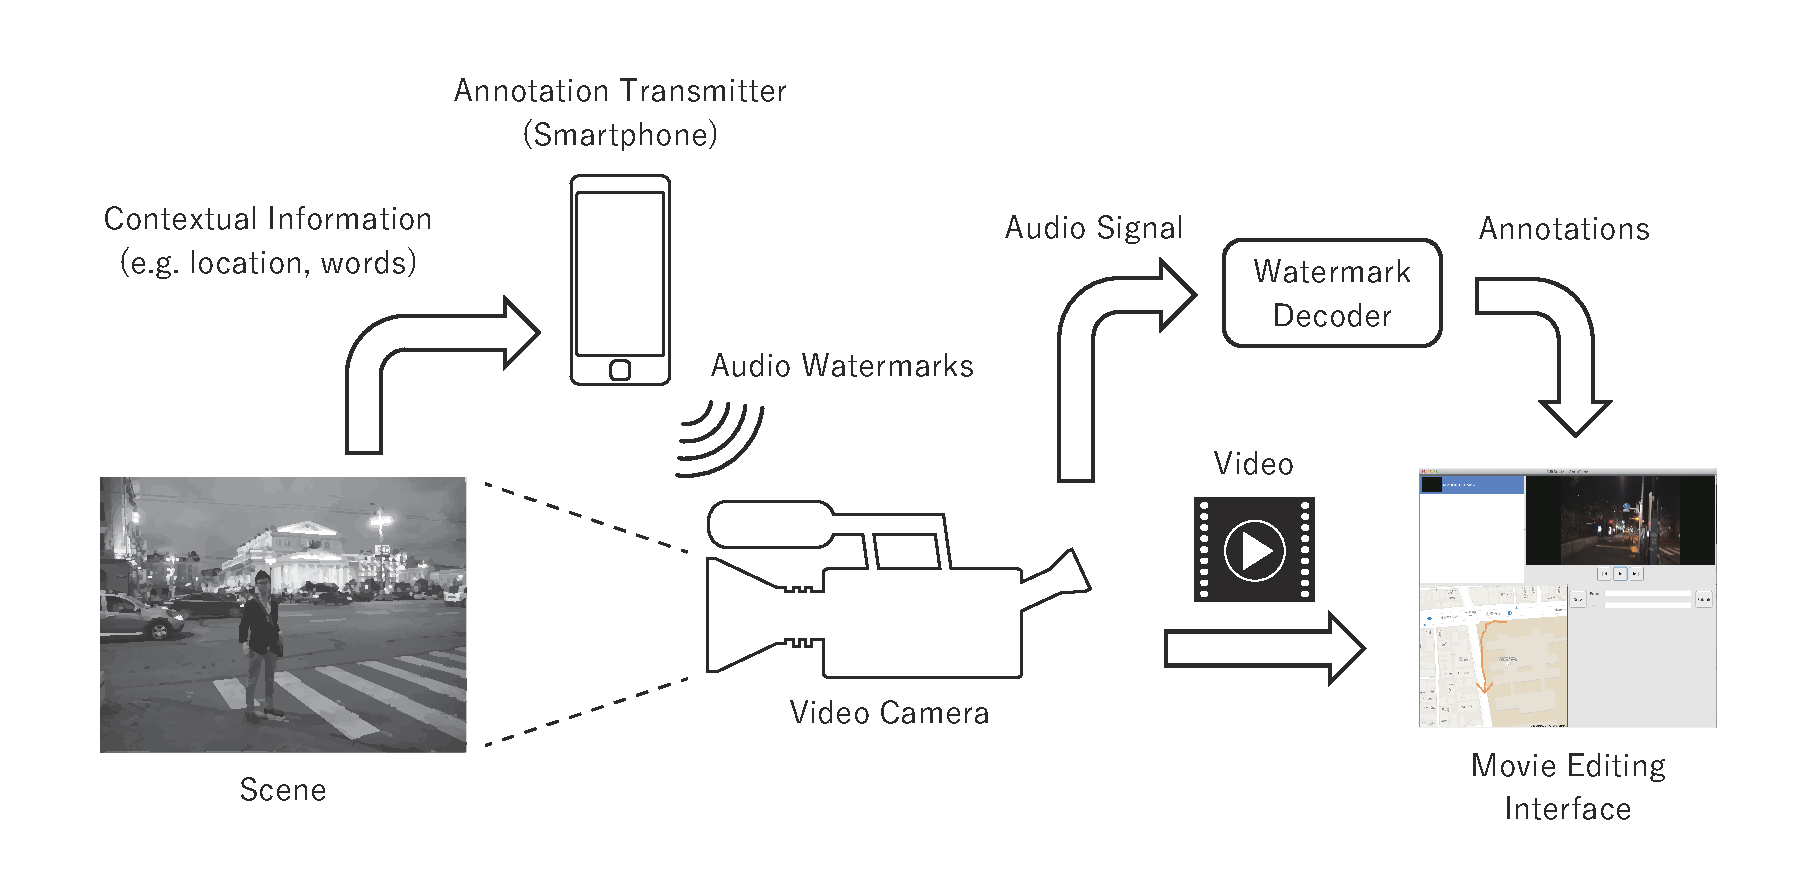
\includegraphics[width=135mm]{overview.pdf}
 \end{center}
 \caption{The schematic diagram of the system of AnnoTone}
 \label{fig:one}
\end{figure}
